\documentclass[11pt]{article}
\usepackage[margin=1in]{geometry}
\usepackage{volfit_preamble}
\graphicspath{{figures/}}

\title{\textbf{SVI-JW: One Hyperbola, Two Languages}\\[2pt]
\large Raw geometry, trader coordinates, and honest arbitrage control\\[2pt]
\normalsize Vol-Fitter Technical Notes, No.~02 --- alternative draft}
\author{Vol-Fitter}
\date{\today}

\newcommand{\vmin}{\widetilde v}
\newcommand{\wmin}{w_\star}
\newcommand{\kmin}{k_\star}
\newcommand{\betL}{\beta_L}
\newcommand{\betR}{\beta_R}

\begin{document}
\maketitle
% Auto-generated by gen_svi_rewrite.py -- do not edit.
\newcommand{\svirwmaxerr}{5.6e-13}
\newcommand{\svirwnfev}{21}
\newcommand{\svirwjwerr}{3.9e-16}
\newcommand{\svirwgmin}{0.343}
\newcommand{\svirwgminloc}{-0.55}
\newcommand{\svirwwingL}{0.1093}
\newcommand{\svirwwingR}{0.0364}
\newcommand{\svirwcountermin}{0.0116}
\newcommand{\svirwcounterlee}{0.174}
\newcommand{\svirwcounterg}{-0.033}
\newcommand{\svirwcounterk}{0.88}
\newcommand{\svirwrigidrms}{147.6}
\newcommand{\svirwrigidmax}{351.9}
\newcommand{\svirwanalyticms}{1.21}
\newcommand{\svirwfdms}{3.06}
\newcommand{\svirwspeedup}{2.53}
\newcommand{\svirwcostdiff}{2.7e-33}
\newcommand{\svirwhistbefore}{26.3}
\newcommand{\svirwhistafter}{10.2}
\newcommand{\svirwhistspeedup}{2.58}
\newcommand{\svirwhistin}{24.3}
\newcommand{\svirwhistoos}{26.8}
\newcommand{\svirwnodes}{1,576}
\newcommand{\svirwarbold}{20.8}
\newcommand{\svirwarbnew}{9.2}
\newcommand{\svirwlqdarbold}{28.3}
\newcommand{\svirwlqdarbnew}{0.0}
\newcommand{\svirwpenalty}{1000}
\newcommand{\svirwleecap}{2.0}
\newcommand{\svirwrawtable}{\begin{tabular}{lr} \toprule Parameter & Value\\ \midrule $a$ & +0.010625\\ $b$ & +0.072887\\ $\rho$ & -0.500000\\ $m$ & +0.058310\\ $s$ & +0.100995\\ \bottomrule \end{tabular}}
\newcommand{\svirwjwtable}{\begin{tabular}{lr} \toprule Handle & Value\\ \midrule $v$ & +0.042500\\ $\psi$ & -0.250000\\ $p$ & +0.750000\\ $c$ & +0.250000\\ $\widetilde v$ & +0.034000\\ \bottomrule \end{tabular}}


\begin{abstract}
SVI draws one expiry's price-implied total variance as a tilted hyperbola.  That
single picture explains both its durability and its limitations: the curve is
smooth, strictly convex in log-moneyness, linear in both wings, cheap to fit,
and unable to turn twice.  The raw coefficients are excellent computational
coordinates but poor market language.  SVI-JW reads the same curve through five
functionals instead: ATM variance, the ATM slope of total volatility, two
normalized wing coefficients, and minimum variance.  We build the raw formula
from a symmetric toy, derive its geometry, define the JW handles in their
natural units, and prove the full image of the coordinate map.  Away from the
ATM-at-the-minimum stratum the inverse is unique; on that stratum the five
handles omit curvature and infinitely many raw slices share them.  The inverse
denominator is quadratic in the distance to this singular set, which explains
its poor conditioning.  We then separate four statements that are often
conflated: convexity of total variance, positive/Lee-clean wings, non-negative
Black density, and calendar ordering.  In particular, the two production
screens are not a butterfly certificate: the Axel Vogt slice has positive
minimum variance and Lee coefficient \svirwcounterlee, yet reaches
$g=\svirwcounterg$.  Finally we derive the unconstrained calibration map and
analytic Jacobian, trace the optional residual blocks, and run a production
JW$\to$raw$\to$fit$\to$JW laboratory round trip with
\svirwmaxerr\ volatility-basis-point maximum error.  Eight generated figures
make the geometry, singularity, arbitrage gap, calibration check, speed result,
and one-hyperbola rigidity visible rather than merely asserted.
\end{abstract}

\clearpage
\tableofcontents
\clearpage

%======================================================================
\section{One curve, two languages}
\label{sec:rw_problem}

A desk rarely asks for ``more $b$'' or ``less $m$.''  It asks where ATM
volatility is, how steeply the smile leaves ATM, how heavy the put wing is, and
where the smile bottoms.  An optimizer has almost the opposite preference: it
wants a formula that evaluates in one pass, differentiates without numerical
noise, and behaves sensibly outside the quoted strikes.  Raw SVI and SVI-JW are
the two languages that serve those two jobs.

The underlying object is not implied volatility itself.  Fix an expiry date
$T$, let $F_T$ be its forward, and write
\begin{equation}
k=\log\frac{K}{F_T},\qquad w(k)=\text{Black implied total variance at }k.
\label{eq:rw_kw}
\end{equation}
The normalized Black price depends on $k$ and $w$, so $w$ is recovered from a
price without first choosing an annualization clock.  Vol-Fitter keeps two
clocks distinct:
\begin{equation}
I_t(k)=\sqrt{\frac{w(k)}{t}},\qquad
I_\tau(k)=\sqrt{\frac{w(k)}{\tau}}.
\label{eq:rw_two_clocks}
\end{equation}
Here $t$ is calendar year fraction and $I_t$ is the ordinary market IV;
$\tau$ is the event-weighted variance time of Note~11 and $I_\tau$ is the
working IV used by the fit and display paths when that clock is enabled.  At
fixed price, changing the clock changes the annualized number, not $w$.  When
events are disabled, $\tau=t$.  Unless qualified, $I$ below means the working
quantity $I_\tau$.

Raw SVI postulates
\begin{equation}
\boxed{
w(k)=a+b\left\{\rho(k-m)+\sqrt{(k-m)^2+s^2}\right\}.}
\label{eq:rw_raw}
\end{equation}
The width is denoted by $s$ so that $\sigma$ remains available for implied
volatility; the production dataclass calls this field \texttt{sigma}.  The
standard raw tuple is $(a,b,\rho,m,s)$ with
\begin{equation}
b>0,qquad |\rho|<1,qquad s>0.
\label{eq:rw_structural}
\end{equation}
Raw SVI was introduced by Gatheral and became a market standard because its
wings are linear in $|k|$ and the formula is unusually tractable
\cite{Gatheral2004,GatheralJacquier2014}.

\begin{invariant}
\begin{enumerate}[leftmargin=1.6em]
\item Every finite optimizer vector maps to a smooth raw hyperbola satisfying
\eqref{eq:rw_structural}; positivity and no-arbitrage require additional work.
\item The JW handles are exact functionals of that same $w$, not a second model.
Their regular inverse is exact only on the domain proved in
\cref{thm:rw_image}.
\item The coded minimum and Lee rows are configurable soft screens.  They do
not certify non-negative density, and the calendar rows do not certify global
cross-expiry order.
\item Production fits and stores raw SVI.  JW is presently an analytical and
test coordinate system: there is no runtime five-handle entry, bump, or export
workflow.
\end{enumerate}
\end{invariant}

The order of the note follows the mathematics rather than the software menu.
We first understand the hyperbola, then learn to read it in JW coordinates,
then ask when it is a legitimate option smile, and only then fit it.

%======================================================================
\section{Building the raw hyperbola}
\label{sec:rw_geometry}

Start with the symmetric toy
\begin{equation}
w(k)=a+b\sqrt{k^2+s^2}.
\label{eq:rw_toy}
\end{equation}
The constant $a$ lifts the curve, $b$ sets the far-wing steepness, and $s$
rounds the corner.  Replacing $k$ by $k-m$ translates the rounded core.
Adding $b\rho(k-m)$ tilts the two wings in opposite directions.  This gives
\eqref{eq:rw_raw}.  The construction is simple, but it already warns us that
$m$ is merely the centre of the square root: after the tilt, it is not the
minimum.

Put
\begin{equation}
x=k-m,qquad r=\sqrt{x^2+s^2},\qquad q=\sqrt{1-\rho^2}.
\label{eq:rw_short}
\end{equation}
These are the only local abbreviations needed for the raw geometry.

\begin{proposition}[Geometry of one raw slice]
\label{prop:rw_geometry}
Under \eqref{eq:rw_structural}, $w$ is strictly convex and has one minimum:
\begin{align}
w'(k)&=b\left(\rho+\frac{x}{r}\right),
&w''(k)&=\frac{bs^2}{r^3}>0,
\label{eq:rw_derivatives}\\
\kmin&=m-\frac{s\rho}{q},
&\wmin&=a+bsq.
\label{eq:rw_minimum}
\end{align}
Its positive left-wing coefficient and right-wing slope are
\begin{equation}
\betL=b(1-\rho),\qquad \betR=b(1+\rho),
\label{eq:rw_betas}
\end{equation}
in the sense that
\begin{equation}
w(k)=\betL|k|+O(1)\quad(k\to-\infty),\qquad
w(k)=\betR k+O(1)\quad(k\to+\infty).
\label{eq:rw_wings}
\end{equation}
The signed derivative on the left tends to $-\betL$; calling $\betL$ a
``left slope'' always means its positive magnitude.
\end{proposition}

\begin{proof}
Differentiation gives \eqref{eq:rw_derivatives}.  Since $b,s>0$, the second
derivative is positive for every finite $k$, so a stationary point is the
unique global minimum.  Solving $w'=0$ gives $x=-s\rho/q$, hence
$r=s/q$ and \eqref{eq:rw_minimum}.  Finally $r=|x|+o(1)$ in either wing,
which yields \eqref{eq:rw_wings}.
\end{proof}

\begin{figure}[H]
\centering
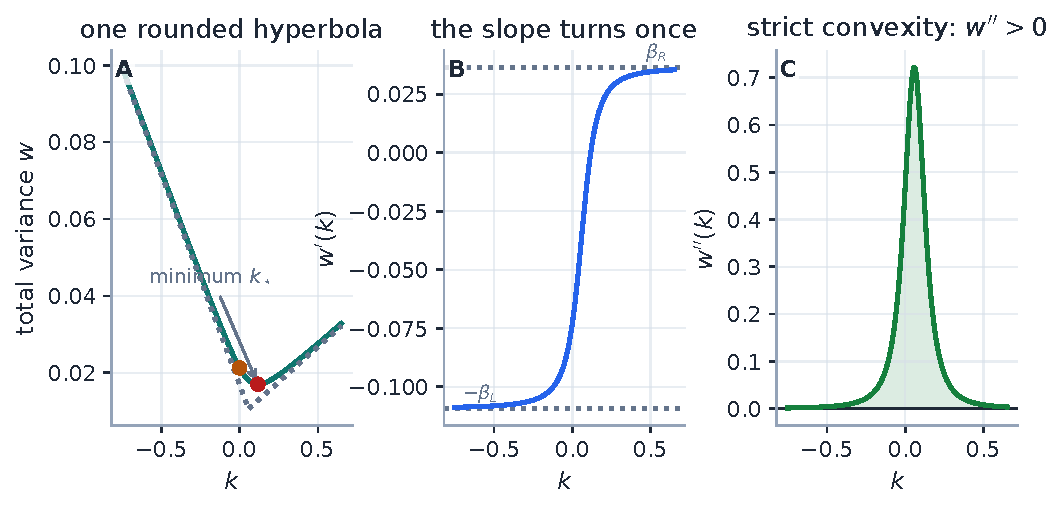
\includegraphics[width=\textwidth]{fig_svi_rewrite_anatomy.pdf}
\caption{One hyperbola carries the entire model.  The total-variance slice
approaches two straight asymptotes (A), its derivative makes one smooth
transition from $-\betL$ to $\betR$ (B), and its curvature is positive
everywhere (C).  The last fact is a geometric statement about $w$; it is not
yet a statement about convexity of option prices.}
\label{fig:rw_anatomy}
\end{figure}

The raw parameters now have a precise, limited interpretation.  Increasing
$a$ is a vertical translation.  Increasing $m$ translates the square-root
core.  But $b$, $\rho$, and $s$ are coupled: $b$ changes the minimum as well as
both wings, $\rho$ changes the minimum location as well as the two wing
coefficients, and $s$ changes both the depth and the breadth of the core.

\begin{figure}[H]
\centering
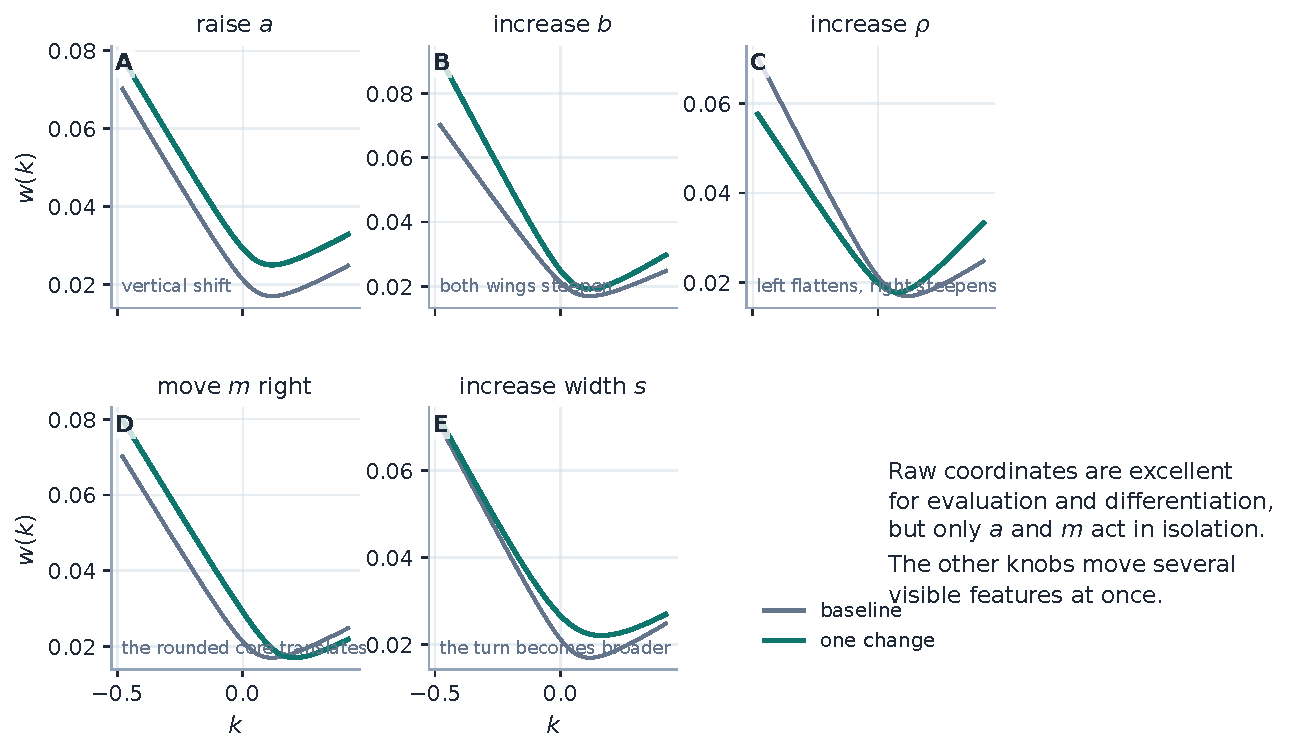
\includegraphics[width=0.98\textwidth]{fig_svi_rewrite_raw_moves.pdf}
\caption{Raw parameters are computational coordinates, not independent market
observables.  Only $a$ is a pure vertical move and only $m$ is a pure
translation of the square-root core.  The other perturbations visibly alter
several features at once, which is the motivation for a second coordinate
chart.}
\label{fig:rw_raw_moves}
\end{figure}

\begin{heuristic}
Think of raw SVI as a rounded hinge.  Far away, the hinge has forgotten its
rounding and exposes two straight rays.  Near the centre, $s$ decides how
quickly one ray turns into the other.  The tilt $\rho$ redistributes a fixed
overall steepness between the put and call sides.  This picture is more useful
than memorizing five coefficient descriptions, but it still does not tell a
trader the ATM level or ATM skew directly.
\end{heuristic}

%======================================================================
\section{Reading the smile: the five JW handles}
\label{sec:rw_jw}

The clean way to introduce SVI-JW is to forget the raw coefficients for a
moment and measure the curve itself.  Let
\begin{equation}
w_0=w(0)>0,qquad \wmin=\min_k w(k).
\label{eq:rw_w0}
\end{equation}

\begin{definition}[SVI-JW functionals]
\label{def:rw_jw}
At variance clock $\tau>0$, the jump-wing coordinates of a smooth raw slice
are
\begin{equation}
v=\frac{w_0}{\tau},\qquad
\psi=\left.\frac{\dd\sqrt{w(k)}}{\dd k}\right|_{k=0},\qquad
p=\frac{\betL}{\sqrt{w_0}},\qquad
c=\frac{\betR}{\sqrt{w_0}},\qquad
\vmin=\frac{\wmin}{\tau}.
\label{eq:rw_jw_functional}
\end{equation}
\end{definition}

This definition separates intrinsic shape from annualization.  The middle
three handles $\psi,p,c$ depend only on the price-derived $w$ and are unchanged
if the clock changes.  Only the annualized levels $v$ and $\vmin$ rescale.
Production uses $\tau$; an external calendar-market convention can replace it
by $t$ without changing the underlying slice.

The displayed meanings follow immediately:
\begin{equation}
I(0)=\sqrt v,qquad I'(0)=\frac{\psi}{\sqrt\tau},qquad
\betL=p\sqrt{v\tau},\qquad \betR=c\sqrt{v\tau},qquad
I(\kmin)=\sqrt{\vmin}\quad\text{if }\vmin\ge0.
\label{eq:rw_jw_display}
\end{equation}
Thus $\psi$ is the ATM slope of \emph{total volatility} $\sqrt w$, or
equivalently $\sqrt\tau$ times the working-IV slope.  The wing handles are
normalized total-variance coefficients, not slopes of the IV plot.

Substituting \eqref{eq:rw_raw} into the functional definition gives the
classical raw-to-JW formulas \cite[Sec.~3.3]{GatheralJacquier2014}:
\begin{equation}
\begin{aligned}
v&=\frac{a+b\{-\rho m+\sqrt{m^2+s^2}\}}{\tau},\\
\psi&=\frac{b}{2\sqrt{w_0}}
       \left(\rho-\frac{m}{\sqrt{m^2+s^2}}\right),\\
p&=\frac{b(1-\rho)}{\sqrt{w_0}},\qquad
c=\frac{b(1+\rho)}{\sqrt{w_0}},\\
\vmin&=\frac{a+bs\sqrt{1-\rho^2}}{\tau}.
\end{aligned}
\label{eq:rw_raw_to_jw}
\end{equation}

\begin{table}[H]
\centering
\small
\begin{tabular}{@{}p{0.08\textwidth}p{0.27\textwidth}p{0.31\textwidth}p{0.24\textwidth}@{}}
\toprule
Handle & Functional definition & What is visible on a chart & Common mistake\\
\midrule
$v$ & $w(0)/\tau$ & ATM IV is $\sqrt v$ & treating $v$ as volatility\\
$\psi$ & $(\sqrt w)'(0)$ & IV tangent is $\psi/\sqrt\tau$ & calling $\psi$ the plotted slope\\
$p$ & $\betL/\sqrt{w_0}$ & put coefficient is $p\sqrt{v\tau}$ & reading it on the IV axis\\
$c$ & $\betR/\sqrt{w_0}$ & call coefficient is $c\sqrt{v\tau}$ & reading it on the IV axis\\
$\vmin$ & $\wmin/\tau$ & minimum IV is $\sqrt{\vmin}$ if non-negative & assuming positivity from the name\\
\bottomrule
\end{tabular}
\caption{The five handles use three related but distinct languages: annualized
variance, total-volatility skew, and normalized total-variance wings.  Keeping
those units explicit prevents nearly every common JW misreading.}
\label{tab:rw_handles}
\end{table}

\begin{figure}[H]
\centering
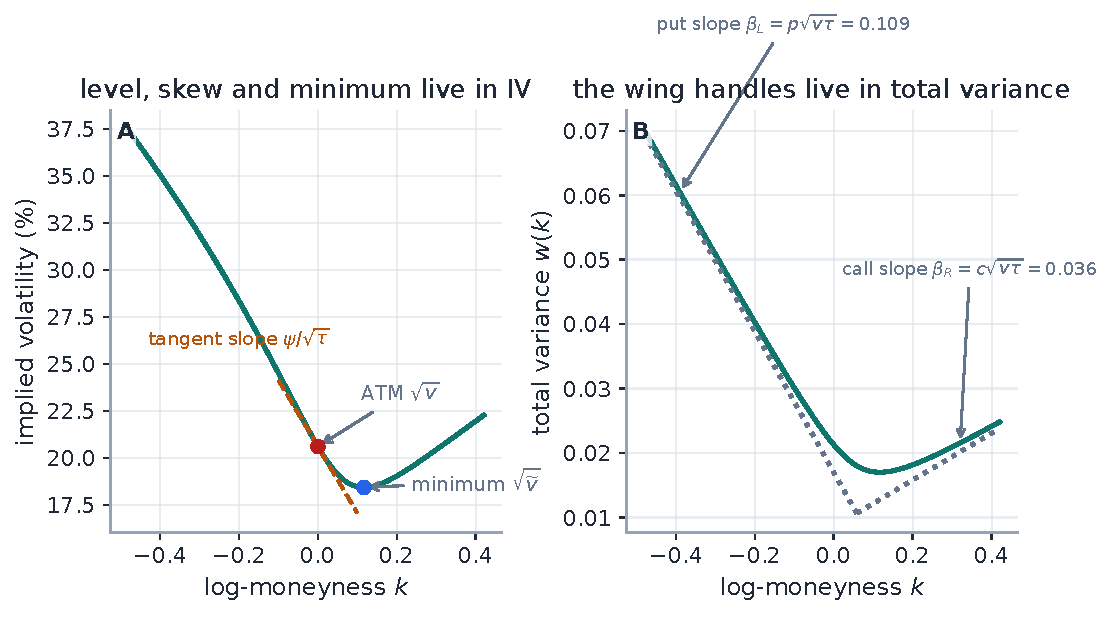
\includegraphics[width=\textwidth]{fig_svi_rewrite_jw.pdf}
\caption{The five JW handles live on two charts.  ATM level, ATM tangent, and
minimum are naturally read in working IV (A).  The put and call handles belong
to the asymptotic total-variance rays (B).  Plotting all five on one IV panel
would give the wing handles units they do not have.}
\label{fig:rw_jw}
\end{figure}

The name ``jump-wing'' is historical trader vocabulary; the five numbers are
not parameters of a jump process.  The parametrization, inspired by a Tim
Klassen coordinate set, was documented alongside the other SVI forms by
Gatheral and Jacquier \cite{GatheralJacquier2014}.  Its value is descriptive:
it turns one opaque coefficient vector into a level, a local slope, two tails,
and a floor.

%======================================================================
\section{Changing coordinates, and where the chart tears}
\label{sec:rw_inverse}

Reading JW from raw is just evaluation.  Going the other way is more
interesting because the five measurements must reconstruct a whole
hyperbola.  Let
\begin{equation}
w_0=v\tau,qquad
\chi=\frac{m}{\sqrt{m^2+s^2}}.
\label{eq:rw_chi}
\end{equation}
The wings first determine the scale and tilt:
\begin{equation}
b=\frac{\sqrt{w_0}}{2}(p+c),qquad
\rho=\frac{c-p}{c+p}.
\label{eq:rw_inv_wings}
\end{equation}
The ATM skew then determines the normalized displacement:
\begin{equation}
\chi=\rho-\frac{4\psi}{p+c}.
\label{eq:rw_inv_chi}
\end{equation}
For $|\chi|<1$, write
\begin{equation}
D(\rho,\chi)=
\frac{1-\rho\chi}{\sqrt{1-\chi^2}}-\sqrt{1-\rho^2}.
\label{eq:rw_D}
\end{equation}
The remaining three raw coordinates are
\begin{equation}
s=\frac{(v-\vmin)\tau}{bD(\rho,\chi)},\qquad
m=\frac{\chi s}{\sqrt{1-\chi^2}},\qquad
a=\vmin\tau-bs\sqrt{1-\rho^2}.
\label{eq:rw_inverse}
\end{equation}
The derivation is only the difference between ATM and minimum variance.  Indeed,
$\sqrt{m^2+s^2}=s/\sqrt{1-\chi^2}$, so subtracting
$\wmin=\vmin\tau$ from $w_0=v\tau$ produces $bsD$.

The factor $D$ has a useful geometric form.  Set
$\rho=\sin\alpha$ and $\chi=\sin\gamma$, with both angles in
$(-\pi/2,\pi/2)$.  Then
\begin{equation}
D(\rho,\chi)
=\frac{1-\cos(\alpha-\gamma)}{\cos\gamma}\ge0,
\label{eq:rw_D_angle}
\end{equation}
and equality holds exactly when $\chi=\rho$.  This one observation supplies
the domain and the singularity.

\begin{theorem}[The full smooth, nondegenerate JW image]
\label{thm:rw_image}
Fix $\tau>0$ and restrict raw SVI to
$b>0$, $|\rho|<1$, $s>0$, and $w_0>0$.

\begin{enumerate}[leftmargin=1.6em]
\item A JW point has a unique regular inverse if and only if
\begin{equation}
v>0,qquad p>0,quad c>0,qquad
-\frac p2<\psi<\frac c2,qquad
\psi\ne0,qquad \vmin<v.
\label{eq:rw_regular_domain}
\end{equation}
On this set, \eqref{eq:rw_inv_wings}--\eqref{eq:rw_inverse} return that inverse.
\item The image also contains the singular stratum
\begin{equation}
v>0,qquad p>0,quad c>0,qquad
\psi=0,qquad \vmin=v.
\label{eq:rw_singular_domain}
\end{equation}
Every point on this stratum is represented by infinitely many raw slices.
There are no other smooth, nondegenerate points in the image.
\end{enumerate}
\end{theorem}

\begin{proof}
If $p,c>0$, \eqref{eq:rw_inv_wings} gives $b>0$ and
$\rho\in(-1,1)$.  Conversely, a smooth raw slice with $b>0$ and
$|\rho|<1$ has $p,c>0$.  From \eqref{eq:rw_inv_chi},
\begin{align*}
|\chi|<1
&\iff \rho-1<\frac{4\psi}{p+c}<\rho+1\\
&\iff -\frac p2<\psi<\frac c2,
\end{align*}
where $(\rho-1)(p+c)=-2p$ and
$(\rho+1)(p+c)=2c$.  This is exactly the condition for finite $m/s$.

By \eqref{eq:rw_D_angle}, $D>0$ precisely when $\chi\ne\rho$, which by
\eqref{eq:rw_inv_chi} is $\psi\ne0$.  The first equation in
\eqref{eq:rw_inverse} then gives $s>0$ precisely when $\vmin<v$.
All remaining coordinates are unique algebraic consequences, proving the
regular statement and its converse.

If $\psi=0$, then $\chi=\rho$.  On a raw slice this is equivalent to
$\kmin=0$ by \eqref{eq:rw_minimum}; hence ATM is the minimum and
$\vmin=v$.  Conversely, fix any $v,p,c$ satisfying
\eqref{eq:rw_singular_domain}.  Equations \eqref{eq:rw_inv_wings} determine
$b,\rho$.  For \emph{any} $s>0$, set
\begin{equation}
m=\frac{\rho s}{\sqrt{1-\rho^2}},qquad
a=v\tau-bs\sqrt{1-\rho^2}.
\label{eq:rw_singular_family}
\end{equation}
Then $\kmin=0$, $\wmin=w_0=v\tau$, and all five JW functionals agree.
The free width proves non-identification.  The preceding necessity arguments
exclude every other smooth nondegenerate case.
\end{proof}

\begin{figure}[H]
\centering
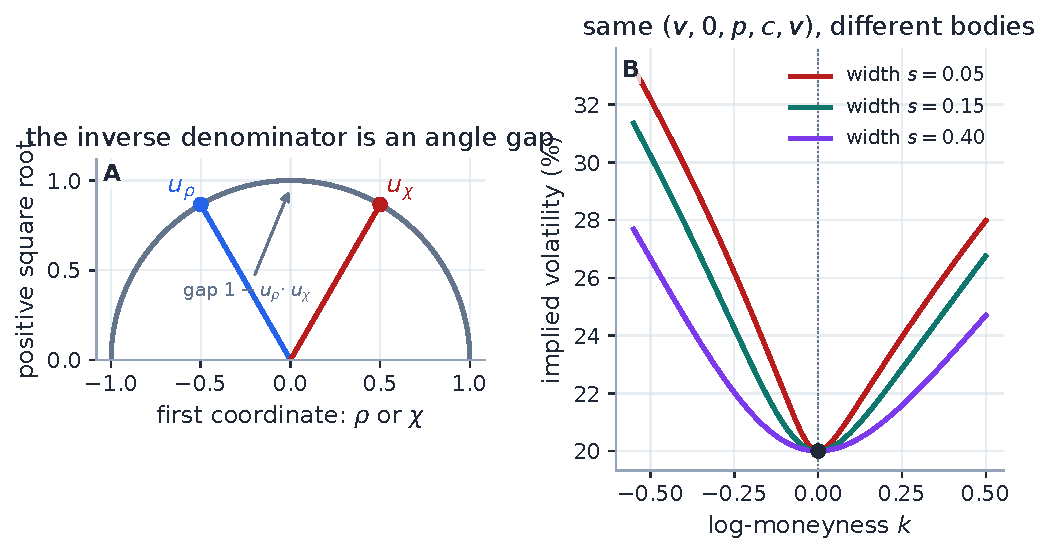
\includegraphics[width=\textwidth]{fig_svi_rewrite_inverse.pdf}
\caption{The inverse denominator measures an angular separation on the unit
semicircle (A).  When the two unit vectors coincide, $\psi=0$ and the chart
loses width information.  Three visibly different raw bodies can then share
the identical tuple $(v,0,p,c,v)$ (B): JW fixes ATM and both asymptotic rays but
omits curvature at the common minimum.}
\label{fig:rw_inverse}
\end{figure}

\subsection{Boundaries and conditioning}

The theorem distinguishes \emph{representability} from \emph{regular
invertibility}.  The most useful boundary cases are collected here.

\begin{table}[H]
\centering
\small
\begin{tabular}{@{}p{0.30\textwidth}p{0.60\textwidth}@{}}
\toprule
JW boundary & What happens\\
\midrule
$\psi=-p/2$ or $\psi=c/2$ & $|\chi|=1$; no finite smooth displacement $m/s$\\
$\psi=0$, $\vmin=v$ & representable, but infinitely many raw widths\\
$\psi=0$, $\vmin<v$ & no finite smooth raw slice\\
$\psi\ne0$, $\vmin=v$ & $s=0$, the nonsmooth V-shaped boundary\\
$p=0$ or $c=0$ & $|\rho|=1$, a one-wing-degenerate boundary\\
$p=c=0$ & $b=0$, the constant-slice boundary\\
$v=0$ & the normalization by $\sqrt{w_0}$ is undefined\\
$\vmin<0$ inside the regular domain & algebraically invertible, financially unusable\\
\bottomrule
\end{tabular}
\caption{The regular domain is open for a reason.  Equality cases are not one
generic failure mode; they lead to distinct degeneracies.}
\label{tab:rw_boundaries}
\end{table}

Near $\chi=\rho$, the angular gap is quadratic:
\begin{equation}
D(\rho,\chi)
\sim \frac{(\chi-\rho)^2}{2(1-\rho^2)^{3/2}},
\qquad \chi\to\rho.
\label{eq:rw_D_asymptotic}
\end{equation}
Because $\chi-\rho=-4\psi/(p+c)$, the denominator is $O(\psi^2)$.
Holding $v-\vmin>0$ fixed therefore sends $s$ to infinity as
$\psi\to0$; a finite approach to the singular family requires
$v-\vmin=O(\psi^2)$.  The limiting ratio is precisely the curvature
information missing from the five handles.

The form \eqref{eq:rw_D} also subtracts nearly equal numbers.  An exactly
equivalent, more stable evaluation is
\begin{equation}
D(\rho,\chi)=
\frac{(\rho-\chi)^2+
\left(\sqrt{1-\rho^2}-\sqrt{1-\chi^2}\right)^2}
{2\sqrt{1-\chi^2}},
\label{eq:rw_D_stable}
\end{equation}
with the square-root difference rationalized in code.  This removes avoidable
cancellation but cannot restore a coordinate that the handles do not identify.

\begin{caution}
The production \texttt{jw\_to\_raw} function implements the direct formulas
without domain guards and has no runtime API/UI caller; tests and document
generators call it with controlled inputs.  Inputs strictly outside the skew
band typically generate NaNs, skew-band endpoints create zero denominators,
and $\vmin\ge v$ returns a degenerate or negative width.  Any future user-facing
JW workflow should validate \eqref{eq:rw_regular_domain}, treat
\eqref{eq:rw_singular_domain} separately, and use a cancellation-resistant
denominator such as \eqref{eq:rw_D_stable}.
\end{caution}

%======================================================================
\section{Convex total variance is not an arbitrage certificate}
\label{sec:rw_noarb}

The phrase ``convex smile'' hides two different derivatives.  Raw SVI has
$w''(k)>0$ by construction.  A butterfly spread, however, tests the second
derivative of an \emph{option price with respect to strike}.  Those statements
are not equivalent.

It helps to keep four levels separate.

\begin{table}[H]
\centering
\small
\begin{tabular}{@{}p{0.20\textwidth}p{0.29\textwidth}p{0.42\textwidth}@{}}
\toprule
Level & Mathematical statement & Production status\\
\midrule
Raw structure & $b>0$, $|\rho|<1$, $s>0$ & hard reparametrization for finite latent coordinates\\
Positive/Lee interior & $\wmin>0$, $\betL<2$, $\betR<2$ & weak closure screened softly: $\wmin\ge0$, $\max(\betL,\betR)\le2$\\
Butterfly clean & non-negative Black density and correct call boundary & measured; not certified by the two core rows\\
Calendar clean & $w_{T_1}(k)\le w_{T_2}(k)$ for every $k$ when $T_1<T_2$ & finite-weight rows on selected grids; not structural\\
\bottomrule
\end{tabular}
\caption{Four increasingly strong meanings of ``valid.''  The first is hard,
the second is softly screened, and the last two require conditions beyond a
single raw coefficient box.}
\label{tab:rw_validity}
\end{table}

\subsection{The exact one-slice criterion}

For normalized strike $y=e^k$, let $\Black(k,w(k))$ be the normalized Black
call and set
\begin{equation}
d_\pm(k)=-\frac{k}{\sqrt{w(k)}}\pm\frac{\sqrt{w(k)}}{2}.
\label{eq:rw_dpm}
\end{equation}

\begin{proposition}[Durrleman's density factor]
\label{prop:rw_durrleman}
Let $w\in C^2(\R)$ be strictly positive.  The strike density implied by the
Black call is
\begin{equation}
\frac{\partial^2\Black}{\partial y^2}
=\frac{\phin(d_-(k))}{y\sqrt{w(k)}}\,g(k),
\label{eq:rw_density_factor}
\end{equation}
where
\begin{equation}
g(k)=
\left(1-\frac{k w'(k)}{2w(k)}\right)^2
-\frac{w'(k)^2}{4}\left(\frac{1}{w(k)}+\frac14\right)
+\frac{w''(k)}{2}.
\label{eq:rw_g}
\end{equation}
Consequently density non-negativity is equivalent to $g(k)\ge0$ for every
$k$.  A standard no-butterfly smile additionally needs the far-call boundary
\begin{equation}
\lim_{k\to+\infty}d_+(k)=-\infty,
\label{eq:rw_call_boundary}
\end{equation}
equivalently the normalized call tends to zero at infinite strike.
\end{proposition}

\begin{proof}
Twice differentiating the Black call with the chain rule gives
\eqref{eq:rw_density_factor}; the prefactor is strictly positive, so its sign
is the sign of $g$.  The boundary is separate because a non-negative local
density need not have the correct total mass or first moment.  This is the
standard Durrleman/Gatheral--Jacquier criterion
\cite{Durrleman2010,GatheralJacquier2014}.
\end{proof}

For raw SVI, Lee's wing bound appears directly in $g$.

\begin{proposition}[Raw-SVI tail limits]
\label{prop:rw_g_tails}
For a structurally valid positive raw slice,
\begin{equation}
\lim_{k\to-\infty}g(k)=\frac{4-\betL^2}{16},qquad
\lim_{k\to+\infty}g(k)=\frac{4-\betR^2}{16}.
\label{eq:rw_g_tails}
\end{equation}
Moreover \eqref{eq:rw_call_boundary} holds exactly when $\betR<2$;
at $\betR=2$, raw SVI has $d_+(k)\to0$.
\end{proposition}

\begin{proof}
In either wing $w\sim\beta|k|$, $|w'|\to\beta$, and $w''\to0$.
The first term of \eqref{eq:rw_g} tends to $1/4$ and the second to
$\beta^2/16$, giving \eqref{eq:rw_g_tails}.  On the right,
\[
d_+(k)=\sqrt{k}\left(-\frac{1}{\sqrt{\betR}}
+\frac{\sqrt{\betR}}{2}\right)+o(\sqrt{k}),
\]
whose coefficient is negative exactly for $\betR<2$.  When $\betR=2$,
the leading terms cancel and the raw linear asymptotic gives the stated zero
limit.
\end{proof}

The strict inequalities are the clean theoretical interior.  The production
hinges use the weak closure because numerical penalties need a boundary.
Similarly, the theoretical positive-smile condition is $\wmin>0$.  A smooth
nondegenerate raw slice touching zero at one finite strike is not a harmless
edge case; it lies outside the butterfly-free raw-SVI domain
\cite{MartiniMingone2022}.  The coded condition $\wmin\ge0$ is a screen, not a
theorem.

\subsection{What the two coded screens look like in JW coordinates}

\begin{proposition}[Core screens in JW units]
\label{prop:rw_screens_jw}
The minimum and Lee quantities satisfy
\begin{equation}
\wmin=\vmin\tau,qquad
\max(\betL,\betR)=\max(p,c)\sqrt{v\tau}.
\label{eq:rw_screens_jw}
\end{equation}
Thus the production weak screens are
$\vmin\ge0$ and
$\max(p,c)\sqrt{v\tau}\le\beta_{\max}$, with default
$\beta_{\max}=\svirwleecap$.
\end{proposition}

\begin{proof}
The first identity is the definition of $\vmin$.  The second follows from
$p=\betL/\sqrt{w_0}$, $c=\betR/\sqrt{w_0}$, and $w_0=v\tau$.
\end{proof}

The screens are necessary ingredients, not sufficient ones.  The sharpest
way to see the gap is a slice that passes both.

\begin{example}[title={Case file: the slice that looks innocent}]
Axel Vogt's counterexample, reproduced as Example~3.1 by Gatheral and Jacquier
\cite{GatheralJacquier2014}, has
\[
a=-0.0410,\quad b=0.1331,\quad \rho=0.3060,\quad
m=0.3586,\quad s=0.4153.
\]
Its minimum total variance is \svirwcountermin, and its larger Lee coefficient
is only \svirwcounterlee.  Both production core screens pass comfortably.
Nevertheless $g$ reaches \svirwcounterg\ near $k=\svirwcounterk$, so the
Black density is negative there.  Strict convexity of $w$ has not protected
strike convexity of the call price.
\end{example}

\begin{figure}[H]
\centering
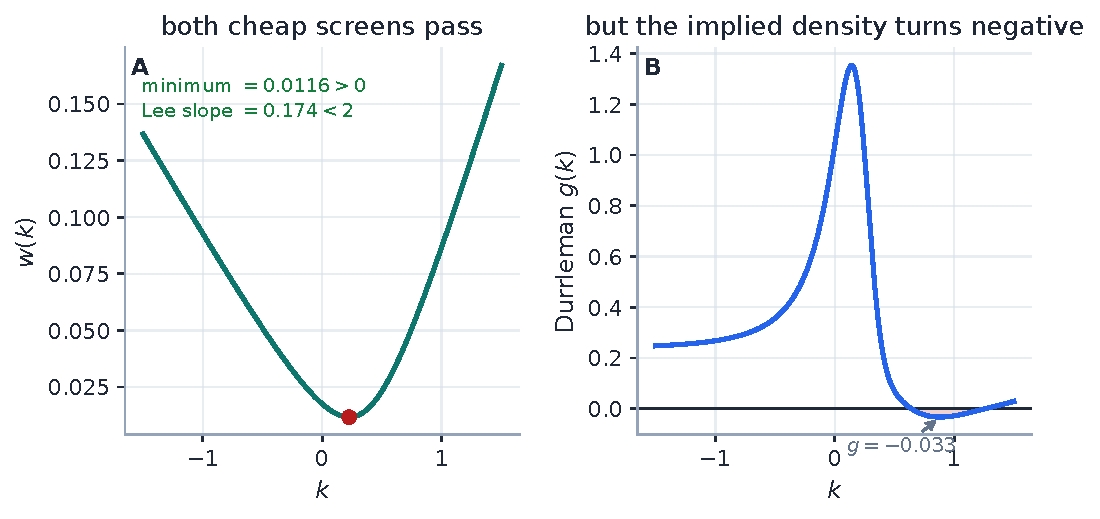
\includegraphics[width=\textwidth]{fig_svi_rewrite_arbitrage.pdf}
\caption{The counterexample is the note's main honesty check.  Its positive,
smooth, strictly convex total variance passes the minimum and Lee screens (A),
while Durrleman's density factor becomes negative (B).  The cheap screens
control common failures; they do not characterize the butterfly-free domain.}
\label{fig:rw_arbitrage}
\end{figure}

Martini and Mingone give a full characterization of the no-butterfly raw-SVI
domain \cite{MartiniMingone2022}.  It is exact but not a single short inequality:
the practical test involves parameter rescaling, root finding, and numerical
minimization.  Vol-Fitter's current raw-SVI calibrator does not implement that
certified domain.  It instead bounds, measures, and optionally repairs through
four separate layers.

\begin{enumerate}[leftmargin=1.6em]
\item \textbf{Core screens.}  Every fit appends the two minimum/Lee hinge rows
of \eqref{eq:rw_core_rows} below.
\item \textbf{Optional extrapolation enforcement.}  With
\texttt{extrapEnforce} on, tapered rows penalize sampled $g<0$, calendar
crossings against the previous displayed slice, and inconsistent wing order in
the extrapolated region.  Only this small block is finite-differenced.
\item \textbf{Advisory diagnostics.}  The Quality path reports remaining
extrapolated-region violations using model-native quantities: closed-form raw
SVI derivatives here, structural density for LQD, and the SIV diagnostic for
that family.
\item \textbf{Publish-time projection.}  The export path can apply the
model-agnostic discrete wing projection of Note~09 while leaving the fitted core
fixed.
\end{enumerate}

No item in that list silently upgrades the raw fit to a global certificate.
The exact criterion remains \cref{prop:rw_durrleman}; the production layers
state what they sample or alter.

The two core residuals are
\begin{equation}
r_{\rm core}=W
\begin{pmatrix}
[-\wmin]_+\\[2pt]
[\max(\betL,\betR)-\beta_{\max}]_+
\end{pmatrix},
\qquad [x]_+=\max(x,0),
\label{eq:rw_core_rows}
\end{equation}
with default residual multiplier $W=\svirwpenalty$.  Because least squares
squares residuals, the objective coefficient is $W^2$.  The two components do
not even have the same natural unit: one is total variance and one is a wing
coefficient.  $W$ is therefore an engineering multiplier, not a financial
variance weight.  At a strictly feasible point both rows and their Jacobian
rows vanish, so the penalized and unpenalized objectives agree locally.  That
fact does \emph{not} imply identical optimizer paths or bitwise identical fits
for arbitrary data.

%======================================================================
\section{How production fits the slice}
\label{sec:rw_calibration}

The optimizer never works directly with a bounded raw vector.  It receives
$\theta\in\R^5$ and maps
\begin{equation}
a=\theta_1,qquad
b=\operatorname{softplus}(\theta_2),\qquad
\rho=\tanh(\theta_3),\qquad
m=\theta_4,qquad
s=e^{\theta_5}.
\label{eq:rw_reparam}
\end{equation}
For every finite $\theta$ in exact arithmetic, $b>0$, $|\rho|<1$, and $s>0$.
This is the hard structural guarantee.  It says nothing about $\wmin$, $g$, or
calendar order.

\subsection{One residual stack}

Suppose price inversion has produced quote total variances $w_i$ at
log-moneyness $k_i$, with working IVs $I_i=\sqrt{w_i/\tau}$ and non-negative
weights $\omega_i$.  In mid mode the data rows are
\begin{equation}
r_i(\theta)=\sqrt{\omega_i}
\left(\sqrt{\frac{w(k_i;\theta)}{\tau}}-I_i\right).
\label{eq:rw_data_rows}
\end{equation}
The core problem is
\begin{equation}
\min_{\theta\in\R^5}\frac12
\left\|
\begin{pmatrix}
r_{\rm data}(\theta)\\ r_{\rm core}(\theta)\\
r_{\rm calendar}(\theta)\\ r_{\rm optional}(\theta)
\end{pmatrix}
\right\|_2^2.
\label{eq:rw_objective}
\end{equation}
With no optional target the last two blocks are empty.  Bid--ask and haircut
modes replace the mid data rows by a vol-space band hinge plus a small mid
anchor.  The surfaced quote-weight choices are \texttt{equal} and
\texttt{tv\_density}; the low-level calibrator also accepts arbitrary weights,
including vega-squared research weights.

The raw structure does not prevent a trial $a$ from making $w$ negative.  To
keep the IV residual evaluable, the calibration residual floors trial total
variance at $10^{-12}$ inside the square root and sets the derivative to zero
where the floor is active.  The \texttt{RawSVI.implied\_vol} method itself has
no such floor; this is a solver device, not a model definition.

\subsection{A geometric, deliberately rough start}

The initializer sorts the quotes, uses the observed argmin as a seed for $m$,
and estimates two finite-span slopes from the endpoints to the array midpoint.
Those slopes seed $b$ and $\rho$; the width starts at one tenth of the quoted
$k$ span, floored at $0.01$, and $a$ is backed out from the observed minimum
with a small positive floor.  Each transformation in \eqref{eq:rw_reparam} is
then inverted to produce $\theta_0$.

This is an initializer, not an estimator.  The observed argmin is generally an
estimate of $\kmin$, not of raw $m$; the array midpoint need not be ATM on an
uneven or one-sided chain; and finite quoted slopes are not asymptotic wings.
The construction is useful because it usually lands in the correct basin, not
because its intermediate numbers have structural meaning.

\subsection{The analytic Jacobian}
\label{sec:rw_jacobian}

The chain has three layers:
\[
\theta\longmapsto(a,b,\rho,m,s)
\longmapsto w(k)
\longmapsto I(k)
\longmapsto r_i.
\]
With $x$ and $r$ from \eqref{eq:rw_short}, the raw partial derivatives are
\begin{equation}
\frac{\partial w}{\partial(a,b,\rho,m,s)}=
\left(
1,\ \rho x+r,\ bx,\ -b\left(\rho+\frac{x}{r}\right),\
\frac{bs}{r}
\right).
\label{eq:rw_raw_partials}
\end{equation}
The latent-coordinate factors are
\begin{equation}
\frac{\dd b}{\dd\theta_2}=1-e^{-b},\qquad
\frac{\dd\rho}{\dd\theta_3}=1-\rho^2,
\qquad \frac{\dd s}{\dd\theta_5}=s,
\label{eq:rw_latent_factors}
\end{equation}
and the IV factor is
\begin{equation}
\frac{\partial I}{\partial w}
=\frac{1}{2\tau I}=\frac{1}{2\sqrt{\tau w}}.
\label{eq:rw_iv_factor}
\end{equation}
Multiplying these factors gives the data Jacobian without another model
evaluation.  Active hinge rows use the derivative of their linear branch and
inactive rows use zero; at a kink the implementation chooses the inactive
subgradient.  In particular the $|\rho|$ term in the Lee row uses
$\sgn(\rho)$, with the zero subgradient at $\rho=0$.

The analytic module covers the mid or band data block, both core rows, and the
sampled calendar floor.  A var-swap target or persistence-prior block switches
the whole fit to finite differences because those rows are not differentiated
there.  Extrapolation enforcement keeps a hybrid Jacobian: the dominant core
remains analytic and only the small extrapolation block is centrally
finite-differenced.

\begin{table}[H]
\centering
\small
\begin{tabular}{@{}p{0.23\textwidth}p{0.46\textwidth}p{0.20\textwidth}@{}}
\toprule
Residual block & Purpose & Jacobian path\\
\midrule
mid or band data & fit working IV, or stay inside bid--ask/haircut band & analytic\\
minimum and Lee & weak core screens \eqref{eq:rw_core_rows} & analytic subgradient\\
calendar floor & reduce sampled crossings against the nearer expiry & analytic subgradient\\
extrapolation & sampled $g$, calendar, and wing-order hinges & analytic core + FD block\\
var-swap quote & pull replicated fair variance toward a quote & finite-difference fit\\
strike/operator prior & preserve under-observed prior shape or operators & finite-difference fit\\
\bottomrule
\end{tabular}
\caption{Every optional target is expressed in the native currency of raw SVI,
but not every row has yet been differentiated analytically.  ``Analytic'' is a
performance statement, not an arbitrage statement.}
\label{tab:rw_blocks}
\end{table}

\begin{perfbox}
The solver remains Levenberg--Marquardt.  A tested switch to trust-region
reflective was slower on noisy real chains because it took more iterations
through hinge changes; the useful change was the Jacobian, not the optimizer.
On the generated 25-quote case, a warmed median-of-five run measures
\svirwfdms\,ms with finite differences and \svirwanalyticms\,ms analytically,
a \svirwspeedup$\times$ speed-up with objective costs agreeing to
\svirwcostdiff.  The separately recorded spike-regime measurement was
\svirwhistbefore$\to$\svirwhistafter\,ms per real node
($\svirwhistspeedup\times$).  The first number is machine-local and regenerated;
the second is a dated historical benchmark recorded in
\texttt{backend/backtest/FINDINGS\_calibration\_arb.md}.
\end{perfbox}

\begin{figure}[H]
\centering
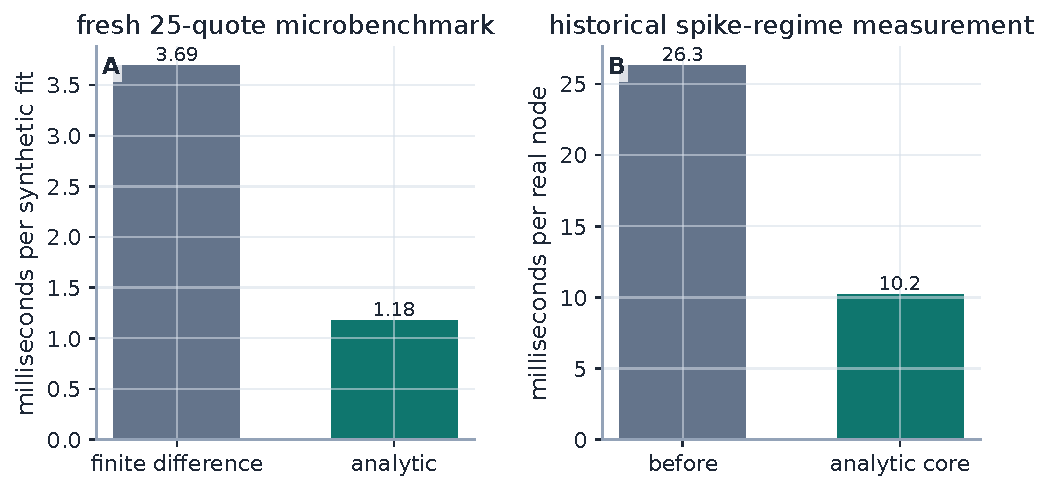
\includegraphics[width=0.95\textwidth]{fig_svi_rewrite_timing.pdf}
\caption{The analytic Jacobian removes repeated residual evaluations rather
than changing the optimizer.  The fresh synthetic timing (A) and the historical
real-node timing (B) have different scales and provenance, but both isolate the
same implementation change.}
\label{fig:rw_timing}
\end{figure}

%======================================================================
\section{Laboratory case: JW to raw to fit to JW}
\label{sec:rw_case}

An exact-family, noise-free recovery is not market evidence.  It is the right
laboratory test for a coordinate conversion and a Jacobian: any visible miss is
an implementation error.

Take $\tau=0.5$ and
\begin{equation}
(v,\psi,p,c,\vmin)=(0.0425,-0.25,0.75,0.25,0.034).
\label{eq:rw_case_jw}
\end{equation}
The production \texttt{jw\_to\_raw} converter builds the target.  We sample 25
noise-free total-variance quotes on $[-0.35,0.30]$, fit production raw SVI from
its geometric start, then read JW back using \eqref{eq:rw_raw_to_jw}.  This is
a genuine
\[
\text{JW}\longrightarrow\text{raw target}
\longrightarrow\text{raw fit}\longrightarrow\text{JW readout}
\]
round trip.

\begin{table}[H]
\centering
\begin{minipage}{0.46\textwidth}\centering
\caption{Recovered raw coordinates.}\label{tab:rw_raw_case}
\svirwrawtable
\end{minipage}\hfill
\begin{minipage}{0.46\textwidth}\centering
\caption{Recovered JW functionals.}\label{tab:rw_jw_case}
\svirwjwtable
\end{minipage}
\end{table}

The maximum quote error is \svirwmaxerr\ vol bp after \svirwnfev\ residual
evaluations.  The maximum absolute JW round-trip error is \svirwjwerr, and the
recovered wing coefficients are \svirwwingL\ and \svirwwingR.  On the plotted
diagnostic grid, $g$ stays above \svirwgmin.  These numbers test algebra and
implementation; they do not measure SVI's ability to fit a non-SVI market.

\begin{figure}[H]
\centering
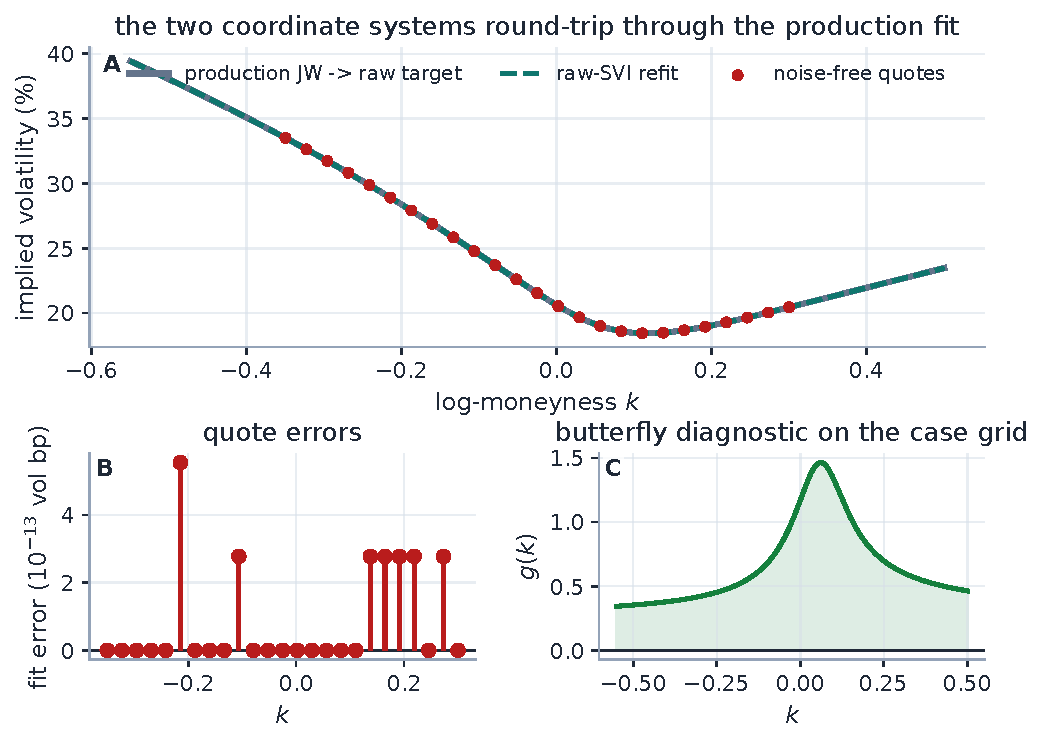
\includegraphics[width=\textwidth]{fig_svi_rewrite_recovery.pdf}
\caption{The laboratory target and fit coincide (A), so the useful evidence is
the residual scale (B) and the independent Durrleman diagnostic (C).  The test
validates conversion, initialization, calibration, and reverse readout in one
reproducible path; it deliberately says nothing about real-market
expressiveness.}
\label{fig:rw_recovery}
\end{figure}

%======================================================================
\section{Where one hyperbola stops being enough}
\label{sec:rw_limits}

Strict convexity of total variance gives SVI one minimum and one transition
between two wing slopes.  This is desirable regularization on sparse equity
index chains, but it is also a hard expressiveness limit.  A W-shaped
total-variance target, a double-humped event density, or a sharply localized
short-dated kink asks the curve to turn more than once.

\begin{figure}[H]
\centering
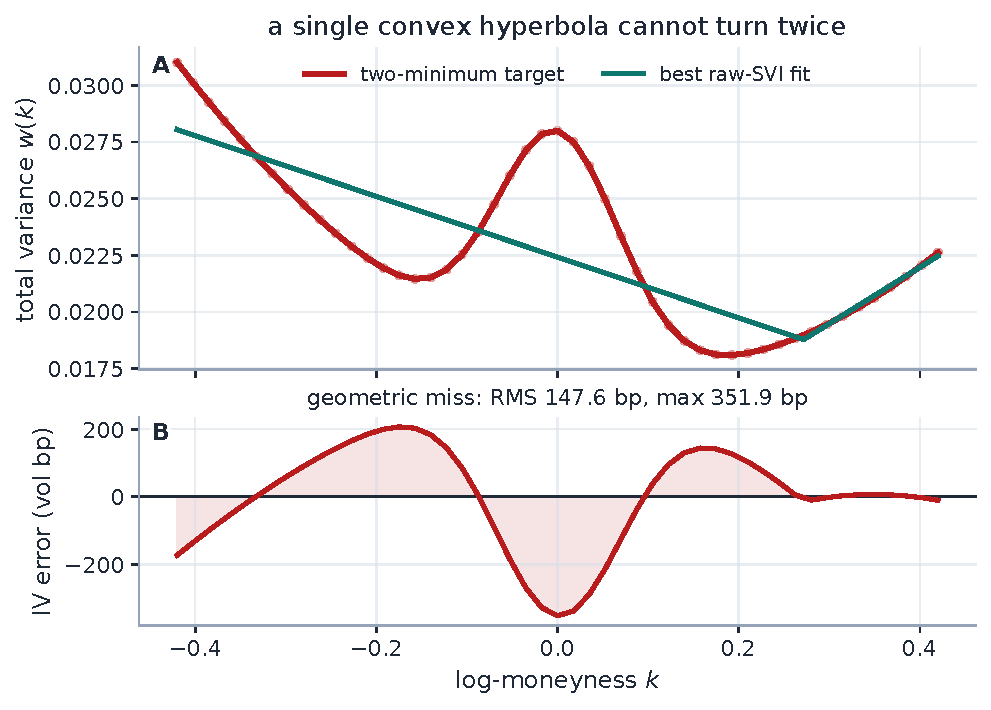
\includegraphics[width=0.96\textwidth]{fig_svi_rewrite_rigidity.pdf}
\caption{A deliberately synthetic positive target has two minima and a central
hump.  Production raw SVI returns the best one-hyperbola compromise (A), leaving
an RMS miss of \svirwrigidrms\ vol bp and a maximum miss of
\svirwrigidmax\ vol bp (B).  This is a geometric stress test, not a claim that
the synthetic target is itself an arbitrage-free market smile.}
\label{fig:rw_rigidity}
\end{figure}

Sparse identification is a different limitation.  On a narrow or one-sided
quote window, distinct raw tuples can price the observed strikes almost
identically while implying different remote wings.  The fitted curve may be
stable even when $(a,b,\rho,m,s)$ is not.  JW is easier to interpret, but its
wing handles are still extrapolated functionals when the market has not quoted
the wings.  Across fits, compare prices, curves, and economically observed
handles before comparing raw coefficients.

The historical spike-regime sweep recorded SVI at \svirwhistin\ vol bp RMS
in-sample and \svirwhistoos\ out-of-sample over roughly \svirwnodes\ nodes per
regime.  Those values are retained for continuity with the current note and
deck, but the underlying result parquets are not checked into this workspace;
they are historical evidence, not a result regenerated by this manuscript.
The same audit changed the SVI butterfly flag rate from \svirwarbold\% under a
reconstructed finite-difference diagnostic to \svirwarbnew\% under the
model-native analytic diagnostic.  The surviving flags are consistent with
the lesson of \cref{fig:rw_arbitrage}: numerical noise exaggerated the old
count, while genuine violations remain possible.

%======================================================================
\section{The honest product and mathematical contract}
\label{sec:rw_contract}

SVI, SVI-JW, and the no-arbitrage analysis are classical.  Raw SVI is due to
Gatheral; the JW chart is documented by Gatheral and Jacquier; Lee supplies the
wing moment bound; Durrleman supplies the density factor; and Martini--Mingone
give the full raw-SVI butterfly domain
\cite{Gatheral2004,GatheralJacquier2014,Lee2004,Durrleman2010,MartiniMingone2022}.

The contribution here is narrower: a clock-consistent derivation in Vol-Fitter
notation, an explicit full-image theorem including the non-identified stratum,
a conditioning analysis tied to the actual converter, a production-accurate
separation of screens from certification, an executable checked reference map,
and traceability from the mathematical claims to code and tests.

\begin{table}[H]
\centering
\small
\begin{tabular}{@{}p{0.30\textwidth}p{0.15\textwidth}p{0.45\textwidth}@{}}
\toprule
Claim or feature & Status & Qualification\\
\midrule
raw SVI evaluation & shipped & runtime model uses \texttt{RawSVI}\\
raw SVI fit and storage & shipped & selected overlay is calibrated and stored in raw coordinates\\
five-handle JW entry/bump/export & not shipped & JW converter is used by tests and document generators, not runtime UI/API\\
raw $\leftrightarrow$ JW equivalence & exact & unique only on \eqref{eq:rw_regular_domain}; singular on \eqref{eq:rw_singular_domain}\\
structural raw inequalities & hard & for finite latent coordinates in exact arithmetic\\
minimum and Lee controls & soft & configurable finite-weight residuals on the weak closure\\
global butterfly freedom & not guaranteed & requires \cref{prop:rw_durrleman}; counterexample is test-locked\\
global calendar freedom & not guaranteed & sampled finite-weight floors reduce crossings\\
one minimum and linear wings & structural & strength for regular smiles, limitation for event/WW shapes\\
analytic core Jacobian & shipped & optional var-swap/prior blocks revert to FD; extrapolation is hybrid\\
\bottomrule
\end{tabular}
\caption{The shortest reliable summary of what the model, coordinate chart,
and implementation do and do not guarantee.}
\label{tab:rw_contract}
\end{table}

%======================================================================
\section{Traceability}
\label{sec:rw_trace}

The table names existing repository anchors.  A test locks only the claim in
its row: selected invalid converter cases do not constitute full input
validation, and a finite diagnostic grid does not constitute a global proof.

\begingroup
\small
\setlength{\tabcolsep}{4pt}
\renewcommand{\arraystretch}{1.13}
\begin{longtable}{@{}p{0.31\textwidth}p{0.14\textwidth}p{0.51\textwidth}@{}}
\caption{Mathematical and production claims with code/test anchors.}\\
\toprule
Claim & Note object & Code and test anchors\\
\midrule
\endfirsthead
\toprule Claim & Note object & Code and test anchors\\ \midrule
\endhead
Clock-independent $w$; production uses working $\tau$ for annualization &
\cref{eq:rw_two_clocks} &
\nolinkurl{api/quotes.py::PreparedQuotes}\newline
\nolinkurl{api/service.py::build_slice_fit_task}\newline
\nolinkurl{api/table.py}\\
\addlinespace
Raw evaluation and production JW$\to$raw conversion &
\cref{eq:rw_raw,eq:rw_inverse} &
\nolinkurl{models/svi_jw/svi.py}\newline
\nolinkurl{tests/test_lqd_pricing.py::test_jw_conversion_matches_note}\\
\addlinespace
Regular round trips and singular $\psi=0$ family &
\cref{thm:rw_image} &
\nolinkurl{models/svi_jw/svi.py}\newline
\nolinkurl{tests/test_svi_domain.py::test_regular_domain_round_trips}\newline
\nolinkurl{::test_psi_zero_stratum_not_identified}\\
\addlinespace
Selected unguarded-converter failure cases &
\cref{tab:rw_boundaries} &
\nolinkurl{tests/test_svi_domain.py::test_invalid_inputs_fail_loudly_not_plausibly}\\
\addlinespace
Minimum/Lee screens do not certify $g\ge0$ &
\cref{fig:rw_arbitrage} &
\nolinkurl{models/svi_jw/calibrate.py::_penalties}\newline
\nolinkurl{tests/test_svi_domain.py::test_core_screens_do_not_certify_butterfly_freedom}\\
\addlinespace
Noise-free raw recovery and curve reproduction &
\cref{sec:rw_case} &
\nolinkurl{models/svi_jw/calibrate.py}\newline
\nolinkurl{tests/test_svi_calibrate.py::test_recovers_benchmark_parameters}\newline
\nolinkurl{::test_curve_reproduced_to_machine_precision}\\
\addlinespace
Analytic Jacobian and active/inactive hinge rows &
\cref{sec:rw_jacobian} &
\nolinkurl{models/svi_jw/jacobian.py}\newline
\nolinkurl{tests/test_svi_jacobian.py}\\
\addlinespace
Band objective reaches SVI &
\cref{tab:rw_blocks} &
\nolinkurl{calib/band.py}\newline
\nolinkurl{tests/test_band_fit.py}\newline
\nolinkurl{tests/test_svi_jacobian.py::test_band_fit_admissible}\\
\addlinespace
Sampled calendar floor and no-floor no-op &
\cref{eq:rw_objective} &
\nolinkurl{models/svi_jw/calibrate.py}\newline
\nolinkurl{tests/test_overlay_calendar.py::test_svi_no_floor_is_byte_identical}\newline
\nolinkurl{::test_svi_floor_crushes_calendar_violation}\\
\addlinespace
Hybrid extrapolation block and advisory measurement &
\cref{sec:rw_noarb} &
\nolinkurl{calib/extrap.py}\newline
\nolinkurl{tests/test_extrap_enforce.py}\newline
\nolinkurl{tests/test_diagnostics.py::test_extrapolated_arb_flags_negative_g_in_wing}\\
\addlinespace
Var-swap target reaches SVI &
\cref{tab:rw_blocks} &
\nolinkurl{calib/varswap.py}\newline
\nolinkurl{tests/test_varswap.py::test_penalty_pulls_model_varswap_toward_quote_all_models}\\
\addlinespace
Operator and strike-anchor priors reach SVI &
\cref{tab:rw_blocks} &
\nolinkurl{calib/operators.py}, \nolinkurl{calib/prior.py}\newline
\nolinkurl{tests/test_prior_parametric.py::test_operator_prior_pulls_all_models_toward_prior_skew}\newline
\nolinkurl{::test_strike_anchor_reaches_svi_and_sigmoid}\\
\addlinespace
Model-native analytic butterfly diagnostic &
\cref{prop:rw_durrleman} &
\nolinkurl{backtest/dispatch.py::_analytic_butterfly}\newline
\nolinkurl{tests/test_backtest_arb.py}\\
\addlinespace
Settings defaults and SVI overlay wiring &
\cref{app:rw_atlas} &
\nolinkurl{api/schemas.py::FitSettings}\newline
\nolinkurl{models/display.py::build_display_fit}\newline
\nolinkurl{tests/test_api_settings.py}\\
\bottomrule
\end{longtable}
\endgroup

\appendix

%======================================================================
\section{Control atlas}
\label{app:rw_atlas}

The table lists direct SVI controls and the shared residual controls that alter
an SVI overlay.  Prior persistence has its own larger atlas in Note~13; the rows
here identify the entry points relevant to this calibrator.

\begin{longtable}{@{}p{0.26\textwidth}p{0.14\textwidth}p{0.53\textwidth}@{}}
\caption{SVI and shared calibration controls.}\\
\toprule Knob & Default & Role\\ \midrule
\endfirsthead
\toprule Knob & Default & Role\\ \midrule
\endhead
\multicolumn{3}{@{}l}{\emph{FitSettings: direct and shared slice controls}}\\
\midrule
\texttt{model} & \texttt{lqd} & Set to \texttt{svi} to display the raw-SVI overlay.\\
\texttt{sviPenaltyWeight} & \svirwpenalty & Residual multiplier $W$ in \eqref{eq:rw_core_rows}; $0$ disables both core screens.\\
\texttt{leeSlopeMax} & \svirwleecap & Weak cap $\beta_{\max}$; values above the theoretical Lee bound are accepted by the schema.\\
\texttt{weightScheme} & \texttt{equal} & Unit or time-value-density quote weights.  Arbitrary low-level arrays are also accepted.\\
\texttt{haircut} & $0.005$ & Absolute-vol tightening used only in haircut band mode.\\
\texttt{midAnchorWeight} & $0.05$ & Small mid anchor appended in bid--ask and haircut modes.\\
\midrule
\multicolumn{3}{@{}l}{\emph{OptionsSettings / request-level shared controls}}\\
\midrule
\texttt{fitMode} & \texttt{mid} & Persisted default: mid, bid--ask band, or haircut band.\\
\texttt{enforceCalendar} & true & Threads the nearer displayed slice into the sampled calendar floor.\\
\texttt{calendarWeight} & $10^6$ & Squared-objective weight; residual rows use its square root.\\
\texttt{extrapEnforce} & false & Adds tapered extrapolation rows and activates the hybrid Jacobian.\\
\texttt{eventsEnabled} & true & Uses event-weighted $\tau$; when the event calendar is empty, $\tau=t$.\\
\texttt{varSwapEnabled} & true & Allows an available variance-swap quote to append its target row.\\
\texttt{varSwapWeightPct} & $10$ & Var-swap budget as a percentage of summed option-quote weights.\\
\texttt{priorPersistenceMode} & \texttt{hybrid} & Routes active transported priors to strike/operator/factor targets; absence of an active prior leaves the blocks empty.\\
\midrule
\multicolumn{3}{@{}l}{\emph{Internal numerical choices}}\\
\midrule
$b=\operatorname{softplus}(\theta_2)$ & --- & Enforces $b>0$ for finite $\theta_2$.\\
$\rho=\tanh(\theta_3)$ & --- & Enforces $|\rho|<1$ for finite $\theta_3$.\\
$s=e^{\theta_5}$ & --- & Enforces $s>0$ for finite $\theta_5$.\\
LM tolerances & $10^{-15}$ & \texttt{xtol}, \texttt{ftol}, and \texttt{gtol}.\\
trial-$w$ floor & $10^{-12}$ & Keeps IV residuals finite on negative-variance trial slices; not part of \texttt{RawSVI.implied\_vol}.\\
\bottomrule
\end{longtable}

%======================================================================
\section{Performance and numerical qualifications}
\label{app:rw_performance}

\begin{enumerate}[leftmargin=1.6em]
\item \textbf{Analytic core.}  The main saving is replacing one base residual
plus five parameter perturbations by one closed-form Jacobian.  The generated
microbenchmark is a warmed median of five timings on the current development
machine; it is a regression signal, not a universal latency number.
\item \textbf{LM rather than trust region.}  LM was retained after matched
experiments on noisy real nodes.  The result is empirical: a different residual
stack or constraint strategy can change the conclusion.
\item \textbf{Conditional acceleration.}  Mid/band, core penalties, and sampled
calendar rows are analytic.  Var-swap and prior rows trigger full finite
differences.  Extrapolation enforcement is hybrid.
\item \textbf{Finite arithmetic.}  The hard map
\eqref{eq:rw_reparam} is exact for finite real inputs.  Floating-point
\texttt{tanh} can round to $\pm1$, exponentials can underflow or overflow, and
$1-e^{-b}$ is less accurate than \texttt{-expm1(-b)} for extremely small $b$.
The production range encountered in ordinary fits stays away from those
extremes; the mathematical statement should nevertheless not be mistaken for
an IEEE-754 proof.
\item \textbf{Low-level input contract.}  The calibrator assumes $\tau>0$,
finite quote arrays, non-negative price-implied total variances, and enough
residual rows for LM.  It does not promise a meaningful five-parameter fit to
an empty, tiny, or one-sided chain, nor global convergence from every start.
\item \textbf{Converter conditioning.}  The checked reference listing below
uses \eqref{eq:rw_D_stable}; it still rejects the singular stratum because no
numerical rearrangement can select a unique missing curvature.
\end{enumerate}

%======================================================================
\section{Executable reference maps}
\label{app:rw_reference}

The following file is imported and executed by
\texttt{figures/gen\_svi\_rewrite.py}.  Before figures are written, its checked
inverse is compared with production \texttt{jw\_to\_raw} on three regular-domain
cases to relative tolerance $2\times10^{-12}$.  The inverse uses the stable
denominator \eqref{eq:rw_D_stable}; the reverse map is exactly the functional
definition \eqref{eq:rw_raw_to_jw}.

\lstinputlisting[caption={Executable raw/JW reference maps used by this note.},
label={lst:rw_reference}]{figures/svi_rewrite_reference.py}

\begin{thebibliography}{9}
\bibitem{Gatheral2004}
J.~Gatheral.
\newblock A parsimonious arbitrage-free implied volatility parameterization
with application to the valuation of volatility derivatives.
\newblock Presentation, Global Derivatives, Madrid, 2004.

\bibitem{GatheralJacquier2014}
J.~Gatheral and A.~Jacquier.
\newblock Arbitrage-free SVI volatility surfaces.
\newblock \emph{Quantitative Finance}, 14(1):59--71, 2014.
\newblock doi:10.1080/14697688.2013.819986.

\bibitem{Lee2004}
R.~W.~Lee.
\newblock The moment formula for implied volatility at extreme strikes.
\newblock \emph{Mathematical Finance}, 14(3):469--480, 2004.

\bibitem{Durrleman2010}
V.~Durrleman.
\newblock From implied to spot volatilities.
\newblock \emph{Finance and Stochastics}, 14(2):157--177, 2010.
\newblock doi:10.1007/s00780-009-0112-1.

\bibitem{MartiniMingone2022}
C.~Martini and A.~Mingone.
\newblock No arbitrage SVI.
\newblock \emph{SIAM Journal on Financial Mathematics}, 13(1):227--261, 2022.
\newblock doi:10.1137/20M1351060.
\end{thebibliography}

\end{document}
